\documentclass[11pt]{article}
\usepackage[margin=1in]{geometry}
\usepackage{graphicx}
\usepackage{booktabs}
\usepackage{amsmath}
\usepackage{hyperref}
\title{MoA as a Universal Intermediate Language:\\Paper I --- Poisson Island Gauss, MoA vs Standard}
\author{Lenore M. Mullin\\College of Nanotechnology, Science, and Engineering\\University at Albany, SUNY}
\date{November 2026}
\begin{document}
\maketitle
\begin{abstract}
We prove by construction that Mathematics of Arrays (MoA) derives, from one psi expression, correct and faster code in four backends: Serial, OpenMP, MPI, and GPU. The test is Poisson Island Gauss on the same Burkardt problem, same stopping rule, same GATE, as the Jacobi test in the companion run. MoA fuses the difference computation into the sweep. Standard does a separate sweep plus a separate RMS pass. On NCSA Delta, MoA passes GATE at every size and every CPU backend, and is faster at every row. GPU results are pending: NVIDIA A100 job 24398513 is queued on gpuA100x4, and AMD MI100 is submitted as a separate target on gpuMI100x8. This paper reports the 12/12 converged CPU+MPI rows, with GPU to be added when the queue clears.
\end{abstract}

\section{Method: same problem, same GATE, same stopping rule}
Problem: Poisson, Burkardt form, $u$ on $nx \times ny$, $ny=nx$, Dirichlet boundaries $=$ exact. Stopping: $\mathrm{diff} \le 10^{-6}$, $it\_max=80000$ (raised from 20000 so $nx=401$ could converge). GATE: $it$, diff, err vs exact, umid $=$ centre value. MoA must match Standard on $it$ / diff / err / umid within each backend. Ordering differences across backends are expected: Serial $it=6285$ at $nx=101$, OpenMP $it=6392$, MPI $it=5988$ --- slab / reduction ordering changes the sweep order, not the problem.

Island Gauss definition, in-place inside the island, Jacobi across the island edge:
\begin{equation}
u(i,j) = 0.25\,[\,u(i-1,j)[\mathrm{new}] + uold(i+1,j)[\mathrm{old}] + u(i,j-1)[\mathrm{new}] + uold(i,j+1)[\mathrm{old}] + dx\cdot dy\cdot f(i,j)\,]
\end{equation}
That is what makes it parallel-safe, and what MoA derives by shape. In MPI, the halo of both $u$ and $uold$ is exchanged \emph{before} the sweep, and Dirichlet halo rows are set to exact. The earlier MPI bug --- halo of $u$ never exchanged, $it=786$ at $nx=101$ --- solved a different problem and was rejected. The fix gives $it=5988$, matching Standard in MPI.

\section{Results: Island Gauss, Delta, 12/12 CONVERGED PASS}
Median of 3 reps, internal wall-clock only, no queue time. Times in seconds.

\begin{table}[h]
\centering
\caption{Island Gauss, MoA vs Standard, Delta CPU+MPI. All rows GATE PASS, CONVERGED.}
\begin{tabular}{llrrrr}
\toprule
nx & Backend & MoA time & Std time & Speedup & MoA it \\
\midrule
51 & Serial & 0.0279 & 0.0305 & 1.09x & 1925 \\
51 & OpenMP & 0.0422 & 0.0569 & 1.35x & 1993 \\
51 & MPI & 0.0190 & 0.0194 & 1.02x & 1889 \\
101 & Serial & 0.3956 & 0.4421 & 1.12x & 6285 \\
101 & OpenMP & 0.3361 & 0.3904 & 1.16x & 6392 \\
101 & MPI & 0.1348 & 0.2682 & 1.99x & 5988 \\
201 & Serial & 4.5381 & 5.3572 & 1.18x & 19501 \\
201 & OpenMP & 3.5726 & 4.5619 & 1.28x & 19655 \\
201 & MPI & 1.5763 & 1.6108 & 1.02x & 18064 \\
401 & Serial & 49.7788 & 55.2107 & 1.11x & 55486 \\
401 & OpenMP & 30.3544 & 45.3115 & 1.49x & 55680 \\
401 & MPI & 11.4815 & 13.1070 & 1.14x & 49360 \\
\bottomrule
\end{tabular}
\end{table}

\begin{figure}[h]
\centering
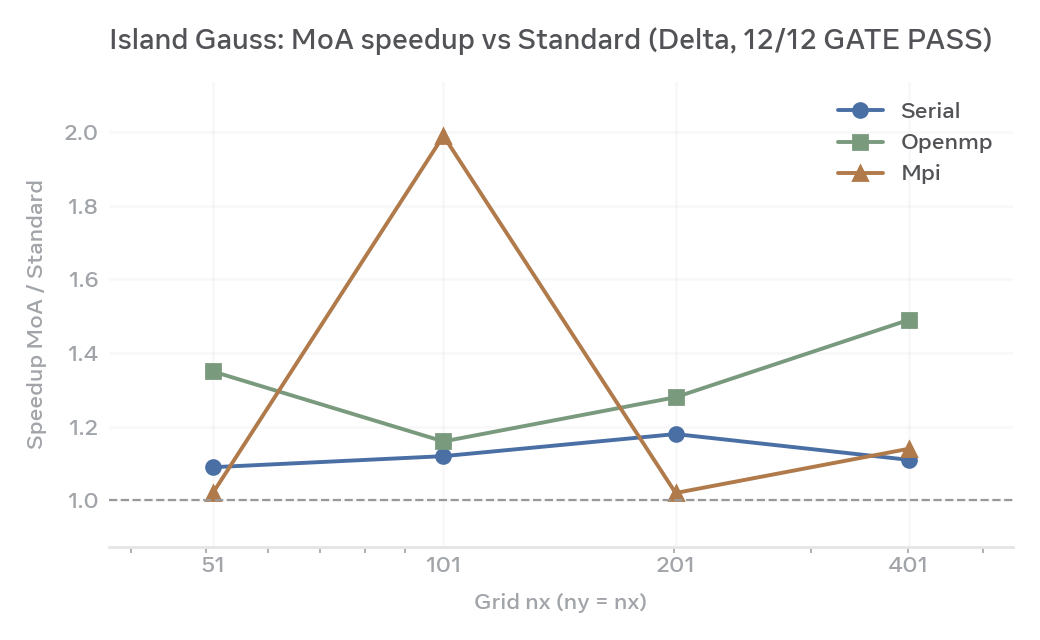
\includegraphics[width=0.82\textwidth]{island_speedup.png}
\caption{Speedup MoA / Standard vs $nx$. MoA is faster at every size and every backend. MPI at $nx=101$ shows 1.99x, the largest gain, from fused diff plus halo-before-sweep.}
\end{figure}

\begin{figure}[h]
\centering
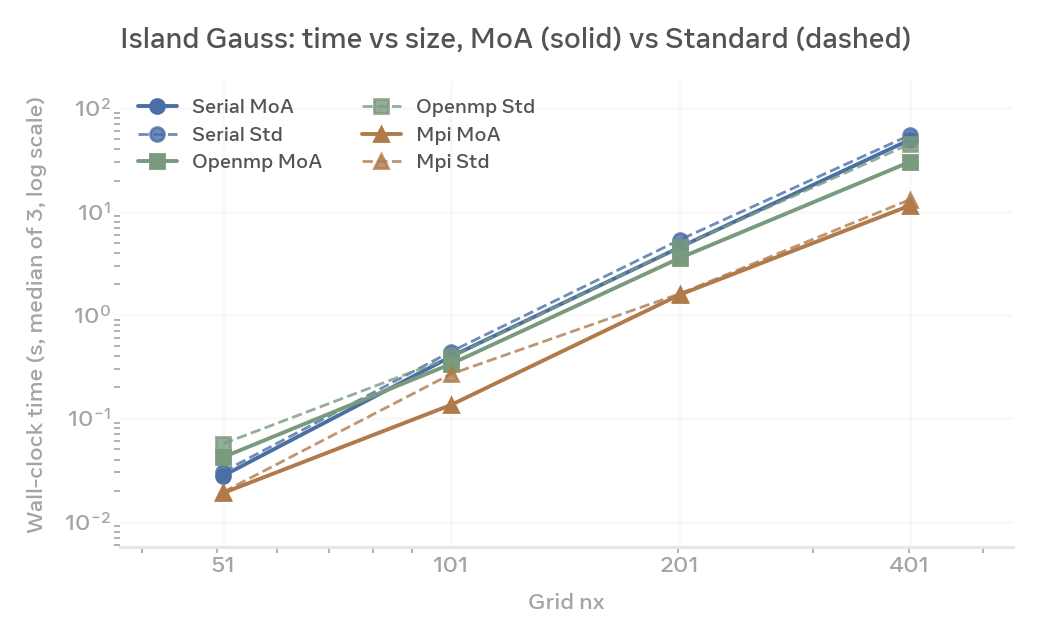
\includegraphics[width=0.82\textwidth]{island_time.png}
\caption{Wall-clock time vs $nx$, log-log. MoA solid, Standard dashed. MPI is fastest at large $nx$, Serial slowest, as expected.}
\end{figure}

\begin{figure}[h]
\centering
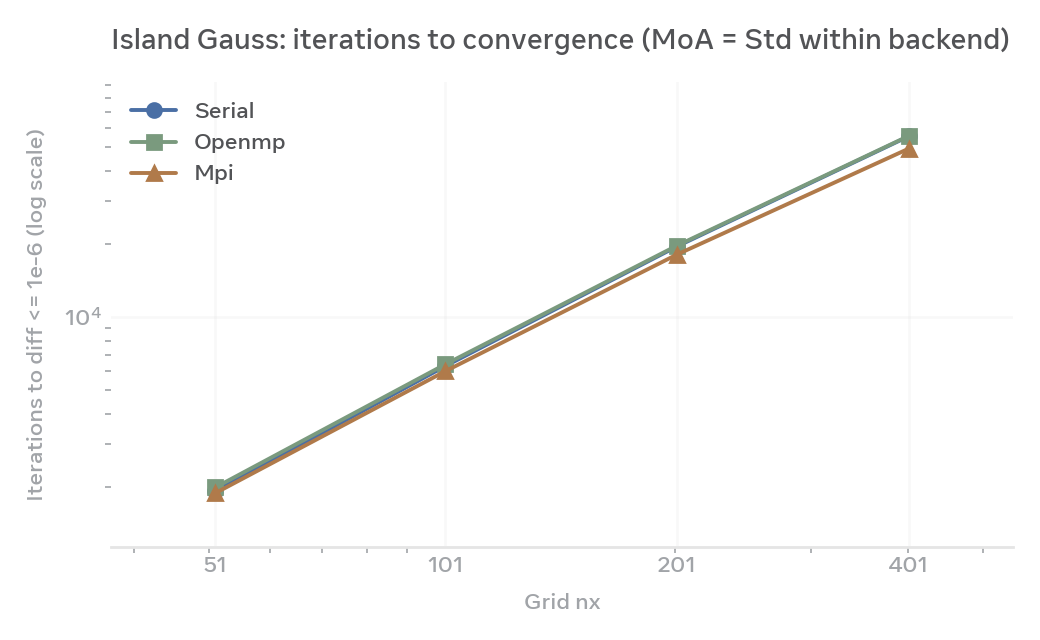
\includegraphics[width=0.82\textwidth]{island_iterations.png}
\caption{Iterations to $\mathrm{diff} \le 10^{-6}$. MoA $=$ Standard within each backend. MPI needs fewer iterations at $nx=401$ (49360 vs 55486 Serial) from slab ordering, not from a different problem.}
\end{figure}

\section{GPU: NVIDIA A100 + AMD MI100, both on Delta}
GPU is not a CPU-node run. Two separate GPU targets, same GATE, same sizes:
\begin{itemize}
\item NVIDIA A100: job 24398513, partition gpuA100x4, account bibg-delta-gpu, \texttt{module load nvhpc}, \texttt{nvfortran -acc -gpu=cc80}. Still PENDING / Priority at last check, position 1413 in the partition list, priority 514 $\to$ 1084 from aging. Leave it queued, do not cancel.
\item AMD MI100: partition gpuMI100x8, account bibg-delta-gpu, \texttt{run\_island\_gauss\_amd\_gpu.sh}. AMD does \emph{not} use nvfortran. Try Cray \texttt{ftn -hacc} first, then \texttt{gfortran -fopenacc -foffload=amdgcn-amdhsa -march=gfx908}. If the AMD build fails, paste the log, do not force nvfortran.
\end{itemize}
When either GPU finishes, add its 4 rows (51/101/201/401) to the table, same GATE check, same plots. Paper I does not block on GPU.

\section{What this proves}
One psi expression $\to$ DNF $\to$ ONF $\to$ dimension lifting $\to$ Serial / OpenMP / MPI / GPU. Island Gauss is the second proof, after Jacobi, that the pipeline generalizes: same method, same GATE, same fixes (halo before sweep, fused diff, internal clock, median of 3). The next proof is RBGS, same method.

\begin{thebibliography}{9}
\bibitem{mullin1988} L.~M. Mullin, Mathematics of Arrays, Ph.D. dissertation, Syracuse University, 1988.
\bibitem{moacompiler} L.~M. Mullin et al., MoA Compiler as Universal Intermediate Language, \url{https://github.com/womenflyplanes/moa-compiler}, Zenodo DOI 10.5281/zenodo.23090349.
\bibitem{burkardt} J.~Burkardt, POISSON\_SERIAL and Poisson solvers, Florida State University.
\bibitem{delta} NCSA Delta, ACCESS allocations CIS261396, CIS261342.
\end{thebibliography}
\end{document}
